%%%%%%%%%%%%%%%%%%%%%%%%%%%%%%%%%%%%%%%%%%%%%%%%%%%%%%%%%%%%%%%%%%%%%%%%%%
 %																		%
 %	Plantilla Latex para presentación del proyecto de curso				%
 %	Programación de Aplicaciones para Internet y la Nube					%
 %																		%
 %	Creada por: Duván Pardo, Wilson López
 % Modificada por: Pedro J. Vargas Barrios								%
 %																		%
 %	Versión: 0.2															%
 %	pedrojvar@gmail.com							%
 %																		% 
 %	Se requieren los archivos  presentación.bbl							% 
 %	El directorio Imagenes que contiene: escudoud.pdf,ECHO_OFF	 		%  
 %																		%
%%%%%%%%%%%%%%%%%%%%%%%%%%%%%%%%%%%%%%%%%%%%%%%%%%%%%%%%%%%%%%%%%%%%%%%%%%

\documentclass[11pt]{beamer}					% Describe el tipo de documento, y el tamaño de la letra del texto
\usepackage[utf8]{inputenc}					% Define codificación para que permita caracteres latinos (acentos)
\usepackage[spanish,activeacute]{babel} 		% Paquete para poder escribir con tildes y otros caracteres especiales

\usepackage{amsmath}							% paquete para expresiones matemáticas
\usepackage{amsfonts}						% paquete para escritura de ecuaciones 
\usepackage{amssymb}							% paquete para caracteres especiales para ecuaciones 

\usepackage{svg}								% Se utiliza para incluir imágenes vectorizadas en el documento (.pdf)
\usepackage{hyperref}						% Para hipervinculos

\usepackage{lmodern}							% http://ctan.org/pkg/lm
\usepackage{listings}						% Para el código fuente
\usepackage{xcolor}							% Para el color en código fuente
\usepackage{graphicx}						% Para incluir imágenes
\graphicspath{{Imagenes/}}					% Directorio de imágenes

\bibliographystyle{apalike} 					% Bibliografia tipo APA

\definecolor{limegreen}{RGB}{50,100,50}		% Definición de color
\lstdefinestyle{base}{						% Para el color en código fuente
	language=C,
	emptylines=1,
	breaklines=true,
	showspaces=fasle,
	showstringspaces=false,
	extendedchars=true,
	basicstyle=\ttfamily\color{black},
	moredelim=**[is][\color{limegreen}]{'}{'},
	moredelim=**[is][\color{blue}]{&}{&},
}				
\lstset{numbers=left, numberstyle=\tiny, stepnumber=1, numbersep=5pt}	% Muestra numeración al lado del código

\mode<presentation>{	
	\usetheme{Frankfurt}		
% Temas: AnnArbor,Antibes, Bergen, Berkeley, Berlin, Boadilla, boxes, CambridgeUS, Copenhagen, Darmstadr, default, Dresden, Frankfurt*, Goettingen, Hannover, LLmenau, JuanLesPins, Luebeck, Madrid, Malmoe, Marburg, Montpellier, PaloAlto, Pittsburgh, Rochester, Singapore, Szeged, Warsaw.	
	\usecolortheme{orchid}	
% Colores:albatross, beaver, beetle, crane, default, dolphin, dove, fly, lily, orchid*, rose, seagull, seahorse, sidebartab, structure, whale, wolverine.	 
}

\logo{
\includegraphics[scale=0.04]{escudoud}}
\title{Handbook Data Centers \\ --- \\ Efficient Hardware-Supported Synchronization Mechanisms for Manycores}
\author{Estudiante(s): Pedro J. Vargas Barrios}
\institute[UD]{Universidad Distrital Francisco José de Caldas}
\date{\today}

\begin{document}	
	
	\begin{frame}[fragile]							% Diapositiva Presentación
		\titlepage 
		\begin{small}
			''Hardware eficiente apoyado en
mecanismos de sincronización para Manycores''
		\end{small}
	\end{frame}	

    	\begin{frame}[fragile]							% Diapositiva Tabla de Contenido
		\frametitle{Índice}	
		\tableofcontents
	\end{frame}	

\section{Introducción}
		 \begin{frame}[fragile]						% Primera Diapositiva
			\frametitle{Introducción}
			\begin{huge}
			\begin{center}
				\emph{\textit{Introducción}}
			\end{center}
			\end{huge}
Los Centros de Datos están evolucionando debido a la necesidad de acoger aplicaciones
distribuidas y en paralelo en ellos, tales como: servicios de computación en
nube, transmisión de vídeo o redes sociales.\\
\begin{figure}[ht] % Es preferible verificar la documentación para que la imagen quede correctamente segun el parámetro entre []
	\centering
		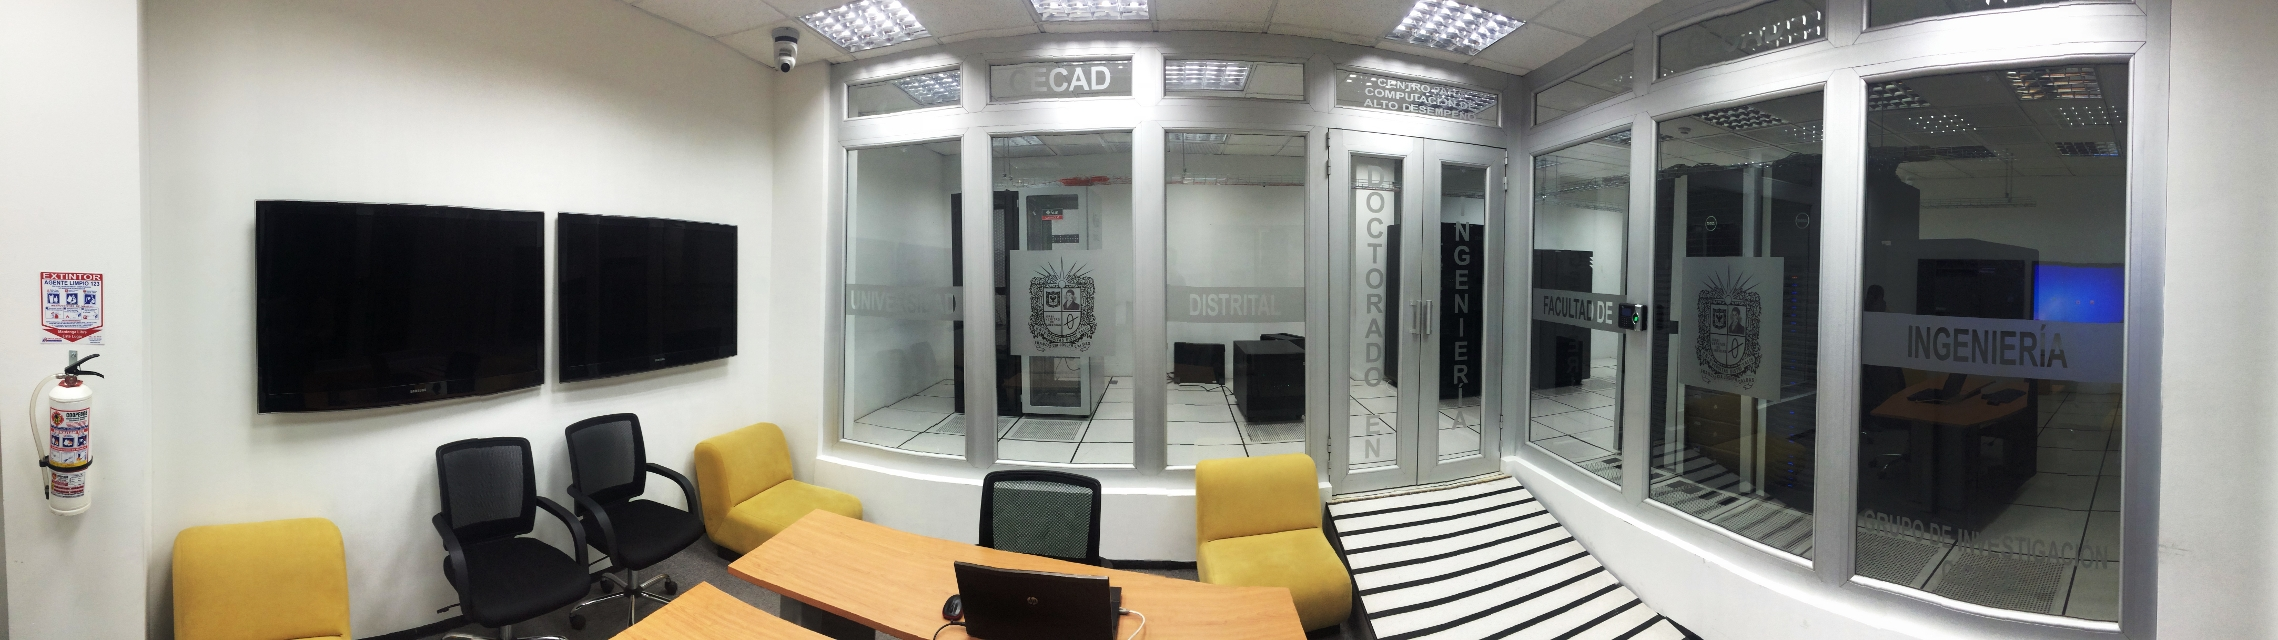
\includegraphics[scale=0.07]{imagenes/cecad.jpg}   % Scale se utiliza para cambiar el tamaño de la imagen
	\caption{CECAD UDistrital} \label{fig:CECAD UDitrital}
\end{figure}
Las arquitecturas Manycore surgen como respuesta a los mayores requerimientos de cómputo; estos son sistemas especialmente adaptados a la explotación de rendimiento masivo.
				
		\end{frame}	

			
\section{Lineas de tecnología G}	
		 \begin{frame}[fragile]
			\frametitle{Lineas de tecnología G}
			\begin{huge}
			\begin{center}
				\emph{\textit{Lineas de tecnología G}}
			\end{center}
			\end{huge}
		\end{frame}		
		   		
    		\subsection{Procesadores}			
			\begin{frame}[fragile]
		\frametitle{Tecnologías G}
			
			\begin{block}{Procesadores}
			
			
Procesador multi-core: Combina dos o más procesadores independientes en un solo paquete o circuito integrado (procesadores independientes)\\
Procesador many-core: Aquitectura que multiples núcleos en un solo paquete de procesamiento único. Pueden ser un procesador de multiples núcleos homogeneos o una arquitectura heterogenea de multiples núcleos.

				\end{block}
				
	
			\end{frame}
			
			\subsection{Arquitectura CBarrier}			
			\begin{frame}[fragile]
		\frametitle{Arquitectura CBarrier}
			
			\begin{block}{Arquitectura CBarrier}
			
			
Los Links
son representados con líneas finas negras mientras
que sus controladores se representan mediante cajas
grises. Hay dos tipos de controladores: maestro (M)
y esclavo (S). Este esquema se caracteriza por tener
el mínimo número de etapas de sincronización, una
propiedad deseable para la aceleración de hardware.

				\end{block}
				
	
			\end{frame}
			
			\subsection{Arquitectura CBarrier}			
			\begin{frame}[fragile]
		\frametitle{Arquitectura CBarrier}
			
	\begin{figure}[ht] % Es preferible verificar la documentación para que la imagen quede correctamente segun el parámetro entre []
	\centering
		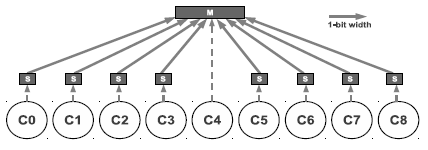
\includegraphics[scale=1]{imagenes/CBarrier.png}   % Scale se utiliza para cambiar el tamaño de la imagen
	\caption{fase gather para CBarrier} \label{fig:fase gather para CBarrier}
\end{figure}
				
	
			\end{frame}
			
\subsection{Arquitectura TBarrier}			
			\begin{frame}[fragile]
		\frametitle{Arquitectura TBarrier}
			
			\begin{block}{Arquitectura TBarrier}
			
			
Proporciona la mejor escalabilidad teórica, debido a
que necesita el menor número de mensajes intercambiados
entre maestro y esclavos. En la imagen se muestran 
tres tipos de controladores: nodos hoja (L), internos (I ) y raíz (R).\\
El controlador R es responsable de contar el
número de participantes. En esta fase, los controladores
L envían un mensaje de un bit a su correspondiente
controlador I. Cuando I ha recibido todos
los mensajes esperados notifica al controlador R.
Finalmente, R espera mensajes de todos los controladores
I.

				\end{block}
				
	
			\end{frame}
			
			\subsection{Arquitectura TBarrier}			
			\begin{frame}[fragile]
		\frametitle{Arquitectura TBarrier}
			
	\begin{figure}[ht] % Es preferible verificar la documentación para que la imagen quede correctamente segun el parámetro entre []
	\centering
		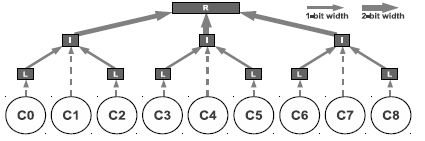
\includegraphics[scale=1]{imagenes/TBarrier.png}   % Scale se utiliza para cambiar el tamaño de la imagen
	\caption{fase gather para TBarrier} \label{fig:fase gather para TBarrier}
\end{figure}
				
	
			\end{frame}
			
			
			
\subsection{Arquitectura GBarrier}			
			\begin{frame}[fragile]
		\frametitle{Arquitectura GBarrier}
			
			\begin{block}{Arquitectura GBarrier}
			
			
En el ejemplo se puede ver que hay cuatro tipos de
controladores: maestros o esclavos horizontales (prefijo
h en la figura) o verticales (prefijo v). las G-Lines
son compartidas por todos los esclavos conectados
a un mismo maestro.\\
simulamos la técnica S-CSMA utilizada en que permite a un controlador
maestro determinar el número de señales desde
los esclavos emitidas de manera simultánea sobre una
G-Line, programando el maestro para que muestre
las señales de todos los enlaces de sus esclavos hasta
que todas las señales esperadas sean recibidas.

				\end{block}
				
	
			\end{frame}
			
			\subsection{Arquitectura GBarrier}			
			\begin{frame}[fragile]
		\frametitle{Arquitectura GBarrier}
			
	\begin{figure}[ht] % Es preferible verificar la documentación para que la imagen quede correctamente segun el parámetro entre []
	\centering
		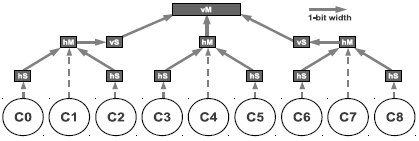
\includegraphics[scale=1]{imagenes/GBarrier.png}   % Scale se utiliza para cambiar el tamaño de la imagen
	\caption{fase gather para GBarrier} \label{fig:fase gather para GBarrier}
\end{figure}
				
	
			\end{frame}			
			
			
			
			
			   		\subsection{Descripción de tecnologías G}			
			\begin{frame}[fragile]
		\frametitle{Tecnologías G}
			
			\begin{block}{Descripción de tecnologías G}
			
			
	Había varias razones que llevaron a utilizar la tecnología
G -Lines para desarrollar mecanismos de sincronizacion de
barreras en los servidores manycore. \\
La
conectividad patron utilizada para desplegar la red de GBarrier
dedicada es basada enlaces unidimensionales de 1 bit que
se integran perfectamente en el concepto de G -Lines

				\end{block}
				
				
	
			\end{frame}
			\section{Hardware de Sincronización Barrier}	
		 \begin{frame}[fragile]
			\frametitle{Hardware de Sincronización Barrier}
			\begin{huge}
			\begin{center}
				\emph{\textit{Hardware de Sincronización Barrier}}
			\end{center}
			\end{huge}
		\end{frame}		
		\subsection{Sincronización Barrier}			
		 \begin{frame}[fragile]						% Primera Diapositiva
			\frametitle{Sincronización Barrier}
			
			\begin{block}{Descripción Sincronización Barrier}
Un Barrier o Barrera es una primitiva de sincronización que
permite que varios procesos o hilos puedan esperar en un punto
de ejecución especial, hasta que todos ellos han llegado a este
antes de que cualquiera de ellos pueda continuar. Un ejemplo
típico de su uso es la utilización de barreras para separar las
diferentes fases que se encuentran comúnmente en aplicaciones
paralelas.			

\end{block}
		\end{frame}
		
				\subsection{Mecanismo de Sincronización GBarrier}			
		 \begin{frame}[fragile]						% Primera Diapositiva
			\frametitle{Mecanisco de Sincronización GBarrier}
			
			\begin{block}{Descripción Mecanismo de Sincronización GBarrier}
Se presenta una propuesta para construir una infraestructura
de hardware eficiente para la sincronización de Barrier en el
contexto de los servidores manycore. Para ello, se comienza
por la descripción de la arquitectura de la red en el chip
dedicado.		

\end{block}
		\end{frame}
		
	\section{Implementación de Tecnologías}	
		 \begin{frame}[fragile]
			\frametitle{Implementación de Tecnologías}
			\begin{huge}
			\begin{center}
				\emph{\textit{Implementación de Tecnologías}}
			\end{center}
			\end{huge}
		\end{frame}		
		\subsection{Implementación de Tecnologías}	
		 \begin{frame}[fragile]	
		 \frametitle{Implementación de Tecnologías}
		Se exponen razones que llevaron a utilizar la tecnología
G -Lines para desarrollar mecanismos de sincronizacion de
barreras en los servidores manycore.\\
En el capitulo se muestran análisis y las propuestas para mitigar el problema de la sincronización a nivel de servidor (procesador Manycore) en centros de datos. Se plantean dos estrategias que proporcionan implementaciones de hardware muy eficientes, escalables y ligeras para barreras (barriers) y bloqueos de contenido.


		
		
		
		\end{frame}
		
	
\section{Bibliografía}	
%BIBLIOGRAFIA 
	\begin{frame}[fragile]
		\frametitle{Bibliografía} 		
        \bibliography{Biblio} 	%Para que aparezca toda la bibliografia que citamos en el documento Biblio.bib, Informe.bbl.
       	\nocite{*}				%Para que aparezca toda la bibliografia que NO citamos en el documento, pero que utilizamos.
	\end{frame}		
				
\end{document}
